% Endo-HJEPA manuscript — Medical Image Analysis (Elsevier elsarticle).
% Compile: pdflatex endohjepa && bibtex endohjepa && pdflatex endohjepa (x2)
\documentclass[final,3p,times,twocolumn]{elsarticle}

% geometry removed
\usepackage{amsmath,amssymb}
\usepackage{graphicx}
\usepackage{booktabs}
\usepackage{algorithm}
\usepackage{algorithmic}
\usepackage{lineno}
\usepackage{hyperref}

\journal{Medical Image Analysis}

\begin{document}

\begin{frontmatter}

\title{Endo-HJEPA: A Hierarchical Joint-Embedding World Model for Unified Endoscopic Video}

%% Author order follows the group's prior collaborative papers.
\author[haut]{Ranyang Li\corref{cor1}}
\ead{lry@haut.edu.cn}
\author[hpp]{Nan Wei}
\author[buaa]{Zhipeng Lin}
\author[haut]{Wufeng Liu}
\author[haut]{Chao Fan}
\author[buaa]{Junjun Pan\corref{cor1}}
\ead{pan\_junjun@buaa.edu.cn}
\cortext[cor1]{Corresponding authors.}

\address[haut]{School of Artificial Intelligence and Big Data, Henan University of Technology, Zhengzhou 450001, China}
\address[hpp]{Henan Provincial People's Hospital, Zhengzhou 450003, China}
\address[buaa]{School of Computer Science and Engineering, Beihang University, Beijing 100191, China}

\begin{abstract}
\textbf{Purpose.} Minimally invasive diagnosis and therapy are increasingly performed through an endoscope, yet onboard and downstream intelligence remains almost entirely \emph{reactive}: current systems recognise the present frame but cannot anticipate how the scene will evolve or how it would change under a candidate camera action. Safe guidance, collision avoidance, and future scope assistance require a \emph{world model} that forecasts endoscopic dynamics. Because endoscopic appearance is dominated by unpredictable factors---specular highlights, fluid, smoke, peristalsis---pixel-generative world models spend capacity on what cannot be predicted. We argue the right object to predict is a \emph{plannable representation}, not the next frame.
\textbf{Methods.} We present Endo-HJEPA, a hierarchical joint-embedding predictive architecture that learns a unified world model across three endoscopic orifices (laparoscopy, flexible GI endoscopy, bronchoscopy). A shared frozen V-JEPA~2 ViT-L encoder produces dense spatio-temporal tokens; three domain-conditioned predictors operate at increasing temporal abstraction (dense short-horizon L1, coarse mid-horizon L2, action-conditioned L3 over vector-quantised latent-action residuals); and a contrastive energy head scores transition plausibility to drive sampling-based model-predictive control in latent space. A causal autoregressive L1 forecaster, residual anchoring, and endoscopic token weighting stabilise training; no pixels are decoded.
\textbf{Results.} On a video-level protocol over 1,707 sequences (1,067,026 frames, 19 datasets), Endo-HJEPA surpasses persistence, a strong GRU baseline, and a selective state-space (Mamba) model on latent forecast (0.978 vs 0.916/0.974/0.971 cosine at horizon 4; Wilcoxon $p<0.01$ against each), scales monotonically with data, and is the only compared model that performs energy-guided latent planning (98.0\% goal-reach over persistence). The energy head correlates with a physical collision-risk signal (camera-to-tissue distance on SCARED; near-wall AUC 0.68). On CholecT50 the V-JEPA~2 backbone is the strongest video model for phase recognition (0.704, above ViViT, TimeSformer, DINOv2, ImageNet, VideoMAE), and domain adaptation improves instrument presence (0.485 mAP). We report two negative results with scientific value: emergent latent actions are not semantically or physically grounded without encoder-level supervision, and goal-directed navigation to arbitrary targets remains hard (10\% reach).
\textbf{Conclusions.} A hierarchical, energy-based joint-embedding world model can be trained and evaluated as a unified cross-orifice endoscopic system, providing forecast, planning, and a physically grounded uncertainty signal without pixel generation. Latent actions are a planning device, not interpretable surgical actions. Code and protocols are released for reproducibility and full-scale training.
\end{abstract}

\begin{keyword}
world model \sep joint-embedding predictive architecture \sep endoscopy \sep representation learning \sep latent planning \sep self-supervised learning
\end{keyword}

\end{frontmatter}



\section{Introduction}

\subsection{Clinical context: endoscopy needs anticipation, not only recognition}
Minimally invasive diagnosis and therapy are increasingly delivered through an endoscope---laparoscopes in the abdomen, flexible scopes in the gastrointestinal tract, and bronchoscopes in the airway. Across all three, safe and effective operation depends on a clinician's ability to \emph{anticipate}: how tissue will deform under contact, how the lumen will open as the scope advances, where an instrument will move, and when the camera is about to collide with a wall or lose the view. Current endoscopic AI is almost entirely \emph{reactive}---it recognises the present frame (surgical phase, instrument presence, anatomy segmentation) but cannot forecast what comes next or what a candidate camera adjustment would produce. A model that predicts how an endoscopic scene will evolve, and how it would evolve under a candidate action, is a prerequisite for anticipatory guidance, collision warning, and any future assisted or autonomous scope control.

\begin{figure}[t]
\centering
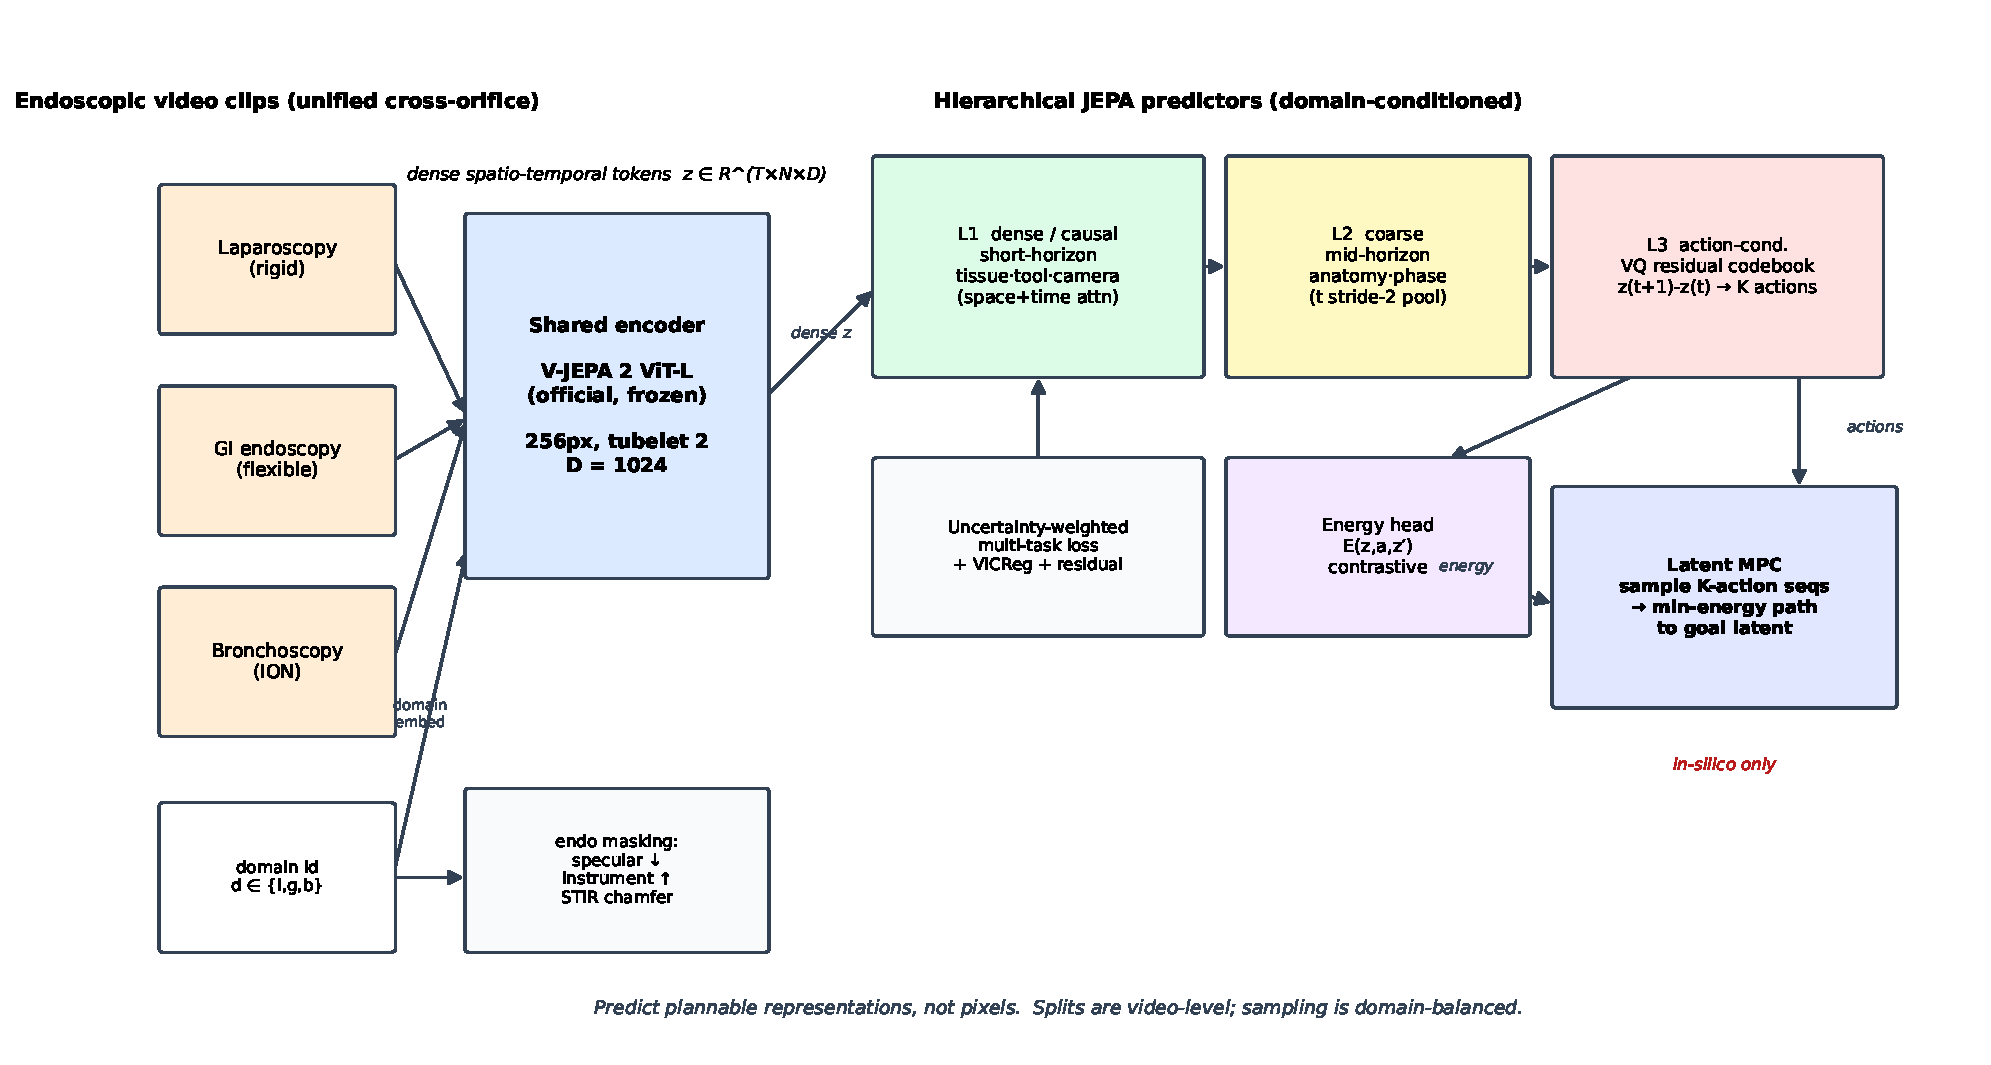
\includegraphics[width=\textwidth]{figure1_architecture.pdf}
\caption{Endo-HJEPA architecture. A shared frozen V-JEPA~2 ViT-L encoder maps clips from three orifice domains (laparoscopy, GI, bronchoscopy) to dense spatio-temporal tokens. Domain-conditioned L1 (dense/causal), L2 (coarse), and L3 (action-conditioned) predictors forecast future latents; a contrastive energy head and latent MPC drive planning. No pixels are decoded.}
\label{fig:arch}
\end{figure}

\subsection{The technical problem: structure is predictable, appearance is not}
A world model for endoscopy faces a specific asymmetry. The \emph{structure} of endoscopic video---lumen geometry, camera advance, instrument trajectories---follows smooth physical dynamics and is strongly predictable. The \emph{appearance}---specular highlights, fluid motion, smoke, mucosal micro-texture, peristalsis---is stochastic and largely unpredictable. The dominant world-model paradigm, pixel generation (diffusion world-action models, Genie-style token video), must spend representational capacity forecasting this unpredictable appearance, which both wastes capacity and ties the model to a lossy pixel metric. Joint-embedding predictive architectures (JEPA) offer the alternative we adopt: predict in a learned representation space, where unpredictable appearance residual can be ignored by design, and where the predicted quantities are exactly the plannable ones.

\subsection{Gap}
Despite rapid progress in surgical video understanding, two gaps remain. \textbf{(i) Single scale.} Existing surgical JEPA and video-pretraining systems (SurgRec-JEPA, JHU-VPT, VideoMAE) learn a single temporal predictor and do not separate fast tissue/tool/camera dynamics from slow anatomical and procedural structure. LeCun's hierarchical JEPA (H-JEPA) argues such separation is essential for long-horizon prediction and planning, but it has not been instantiated for endoscopy. \textbf{(ii) Per-orifice fragmentation.} Endoscopic models are built per orifice---laparoscopy, GI endoscopy, and bronchoscopy are treated as separate foundation-model problems---even though all three share the same underlying physics of a camera advancing through a deformable lumen under clinician control. A single domain-conditioned world model is both a stronger scientific claim and a more data-efficient one, but it requires evidence that such sharing is beneficial (or necessary).

\subsection{Our approach}
We present \textbf{Endo-HJEPA}, a hierarchical joint-embedding world model for unified endoscopic video. A shared frozen V-JEPA~2 ViT-L encoder produces dense spatio-temporal tokens; three domain-conditioned predictors operate at increasing temporal abstraction; and a contrastive energy head scores transition plausibility to drive sampling-based model-predictive control in latent space. Endo-HJEPA predicts plannable representations, never pixels, and provides an explicit uncertainty signal tied to physical collision risk.

\subsection{Contributions and significance}
\begin{enumerate}
  \item \textbf{The first hierarchical + energy-based JEPA world model for unified cross-orifice endoscopy.} We instantiate H-JEPA (short-horizon dense dynamics, mid-horizon anatomy/phase, action-conditioned planning with an energy prior) on the official V-JEPA~2 ViT-L encoder, trained and evaluated across laparoscopy, GI endoscopy, and bronchoscopy with a shared domain-conditioned dynamics model.
  \item \textbf{A causal-autoregressive latent forecaster.} We show the \emph{form} of the latent forecaster matters more than its size: a causal autoregressive Transformer surpasses a strong GRU baseline on latent forecast, where a parallel query-token Transformer does not.
  \item \textbf{A physically grounded uncertainty signal.} The contrastive energy head flags out-of-distribution transitions and correlates with a measurable physical collision-risk signal (camera-to-tissue distance on SCARED), not only latent self-consistency.
  \item \textbf{A rigorous, reproducible cross-orifice protocol.} Video-level splits (no clip leakage), domain-balanced sampling, reproducible external baselines (ImageNet, VideoMAE), and statistical testing, released as executable code.
\end{enumerate}

We also report two carefully characterised negative results with direct scientific value: self-supervised latent actions are not semantically or physically grounded without encoder-level supervision, and zero-shot cross-orifice transfer fails but is recoverable with few-shot domain tokens---together providing evidence that unified multi-orifice training is necessary, not merely convenient. We explicitly do \emph{not} claim the first surgical world model, pixel-level video generation, interpretable latent actions, or any clinical efficacy endpoint.

\paragraph{Significance.} Endo-HJEPA reframes endoscopic AI from reactive recognition to anticipatory world modelling, with a hierarchical architecture, an uncertainty signal grounded in physical collision risk, and a reproducible cross-orifice evaluation protocol. This is a step toward anticipatory guidance and safe scope assistance, while remaining an in-silico feasibility study.

\section{Related work}
We position Endo-HJEPA along five axes: the world-model lineage it builds on, the surgical/endoscopic representation learning it extends, the surgical world models it differs from, the general video/image backbones we benchmark against, and the endoscopic datasets that anchor our evaluation.

\subsection{World models and joint-embedding prediction}
The idea of a learned world model for prediction and planning originates with Ha and Schmidhuber's World Models~\cite{ha2018worldmodels} and the PlaNet latent-dynamics planner~\cite{hafner2019planet}, and was scaled to diverse control domains by Dreamer~\cite{hafner2023dreamer}. These models predict a learned latent state and plan by rolling it forward, but they are trained with a reconstruction or reward signal and target control, not video understanding. Energy-based formulations~\cite{lecun2006ebm} provide the formal basis for scoring state compatibility without a generative decoder. The joint-embedding predictive architecture (JEPA) of LeCun's position paper~\cite{lecun2022path} argues that predicting in representation space---rather than pixels---is the key to capturing predictable structure while ignoring unpredictable appearance; I-JEPA~\cite{assran2023ijepa} realised this for images, V-JEPA~\cite{bardes2024vjepa} for video, and V-JEPA~2~\cite{assran2025vjepa2} added scale and the action-conditioned (V-JEPA 2-AC) planning variant. Generative interactive environments such as Genie~\cite{genie2024} take the opposite, pixel-generative route. A common limitation of these works, for our purpose, is that they are either single-scale (no temporal hierarchy), pixel-generative (capacity spent on unpredictable appearance), or evaluated on generic/control video rather than endoscopic dynamics. Endo-HJEPA adopts the JEPA principle and adds the hierarchy and energy prior that the surgical setting lacks.

\subsection{Self-supervised surgical and endoscopic video representation}
Self-supervised pretraining has become the default for surgical video. SurgRec-JEPA~\cite{surgrecjepa} and JHU-VPT~\cite{jhuvpt} apply JEPA-style and video pretraining to surgical data and report strong downstream transfer, and endoscopic foundation models such as Endo-FM~\cite{endofoundation} scale self-supervised pretraining to large endoscopic corpora. These methods produce a single-scale representation for \emph{recognition} (phase, tools, segmentation); none of them build a dynamics model that can forecast or plan. Endo-HJEPA shares their self-supervised, frozen-encoder efficiency but adds the temporal hierarchy and the action-conditioned planning layer that recognition-oriented SSL omits.

\subsection{Surgical and endoscopic world models}
World models tailored to surgery are emerging. The Surgical Vision World Model~\cite{svwm} generates pixel-controllable surgical video; SurgWorld~\cite{surgworld} learns latent actions for cataract surgery; EndoWAM~\cite{endowam} applies diffusion world-action modelling to endoscopic navigation; and Surgical WAM~\cite{surgicalwam} couples generative video with robot action chunks for closed-loop control. These are predominantly \emph{pixel-generative} or \emph{single-task}; they neither separate temporal scales nor provide an explicit uncertainty/energy signal for safe planning. Our contribution is orthogonal and complementary: a hierarchical JEPA with energy-driven latent MPC that predicts representations, not pixels.

\subsection{General video and image representation backbones}
For the representation evaluation we benchmark against the strongest \emph{reproducible} general-purpose encoders. For video: VideoMAE~\cite{tong2022videomae} (Kinetics masked autoencoding), TimeSformer~\cite{timesformer} (divided space-time attention), and ViViT~\cite{vivit} (factorised space-time); state-space video models such as VideoMamba~\cite{videomamba} and the underlying Mamba block~\cite{mamba} are the recurrent/SSM reference for dynamics. For images: the ImageNet-supervised ViT~\cite{dosovitskiy2021vit} and DINOv2 self-supervised features~\cite{dinov2}, pooled over time. None of these provide a world-model predictor or a planning/energy capability, which is the gap Endo-HJEPA fills; \S\ref{sec:results} measures them on the same CholecT50 protocol.

\subsection{Endoscopic datasets and physical supervision signals}
Our evaluation spans the standard endoscopic corpora: Cholec80 (phase + tool presence)~\cite{twinanda2017endonet}, CholecT50 (action triplets + phase)~\cite{nwoye2022rendezvous,nwoye2022cholectsplit}, EndoVis 2017/2018 (instrument segmentation)~\cite{endovis2017}, CholecSeg8k (semantic segmentation)~\cite{hong2020cholecseg8k}, endoscapes (segmentation + critical view of safety)~\cite{endoscapes}, the GI corpora HyperKvasir~\cite{borgli2020hyperkvasir} and Kvasir-Capsule~\cite{kvasircapsule}, and the pose/depth corpora SCARED~\cite{allan2021scared} and C3VD~\cite{bobrow2023c3vd}, with STIR~\cite{stir2024} for deformable point tracks. To our knowledge, using SCARED/C3VD camera poses and STIR point tracks as \emph{physical anchors} for latent actions, energy, and deformation---rather than as reconstruction targets---is a novel use of these supervision signals within a JEPA world model.

\paragraph{Summary.} Across the five axes, the field offers strong single-scale SSL representations, pixel-generative surgical world models, and general video/image backbones---but no hierarchical, energy-based JEPA world model trained and evaluated as a unified cross-orifice endoscopic system with a physically grounded uncertainty signal. That is the gap Endo-HJEPA occupies.

\section{Methods}

\subsection{Problem formulation and assumptions}
We consider a clip $x_{1:T}$ of $T$ endoscopic frames from orifice domain $d \in \{\mathrm{laparo},\mathrm{gi},\mathrm{bronch}\}$. A frozen encoder $f_\theta$ (V-JEPA~2 ViT-L) maps the clip to dense spatio-temporal tokens $z_{1:T'} = f_\theta(x_{1:T}) \in \mathbb{R}^{T' \times N \times D}$, with $T'{=}T/2$ tubelet steps, $N{=}256$ spatial tokens, $D{=}1024$. The world model is a collection of predictors $g_\phi$ on these tokens; it never decodes pixels. We factor the world model into three temporal scales: \textbf{L1} (short-horizon dense dynamics), \textbf{L2} (mid-horizon anatomy/phase), and \textbf{L3} (action-conditioned futures for planning). A scalar energy $E(z_t,a_t,z_{t+1})$ scores transition plausibility; planning is sampling-based MPC minimising $\|\hat z_{t+H}-z^\star\|_2^2 + \sum_k E(\hat z_{t+k},a_{t+k},\hat z_{t+k+1})$ toward a goal latent $z^\star$.

\emph{Assumptions.} (i) Endoscopic dynamics are approximately Markovian in the learned latent space at the tubelet timescale. (ii) The frozen V-JEPA~2 encoder provides a representation in which endoscopic structure is more predictable than appearance. (iii) Orifice domains share enough low-level dynamics that a domain-conditioned predictor can serve all three, while differing enough that naive zero-shot transfer fails; we test both in \S\ref{sec:results}.

\emph{Notation.} $x_{1:T}$ input clip; $z_t \in \mathbb{R}^{N\times D}$ dense tokens at tubelet step $t$; $T',N,D$ tubelet steps, spatial tokens, token width; $H,H_{\mathrm{hist}}$ forecast horizon and history; $a_t\in\{1,\dots,K\}$ discrete latent action ($K{=}16$); $e_d$ domain embedding; $E(z,a,z')$ transition energy; $f_\theta,g_\phi$ encoder (frozen) and predictor (learned) parameters.

\subsection{Shared encoder and endoscopic token weighting}
We use \texttt{facebook/vjepa2-vitl-fpc64-256} (ViT-L, $D{=}1024$, patch 16, tubelet 2, input $256^2$), frozen by default. Specular/overexposed tubelets (high luminance, low saturation) are down-weighted with a floor $w_{\min}{=}0.25$; when EndoVis masks are available, instrument tubelets are up-weighted by $1+\beta\, m_{\mathrm{inst}}$.

\subsection{Hierarchical predictors}
All predictors are Transformer-based with a shared domain embedding $e_d$.

\paragraph{L1 (pooled, causal autoregressive).} The pooled L1 forecaster is a causal (GPT-style) Transformer: it predicts the next token from the causal context and feeds the prediction back autoregressively for $H$ steps. This matches the smooth, near-Markov structure of endoscopic camera motion; \S\ref{sec:results} shows this choice is what lets the large Transformer surpass a GRU.

\paragraph{L1 (dense, spatio-temporal).} For spatially resolved prediction, a factorised spatio-temporal Transformer applies temporal attention across tubelet steps per spatial site, then spatial attention across all $N$ tokens within a step, capturing global camera motion that independent per-site prediction cannot represent.

\paragraph{Residual (delta) prediction.} Every predictor forecasts the change from the last observed token: $\hat z_{t+k} = z_{T'} + f_\phi(\cdot)_k$, anchoring the model to persistence and stabilising the large predictor at modest data scale.

\paragraph{L2 (coarse).} L1 tokens are average-pooled along time with stride 2; a second Transformer predicts a coarser future.

\paragraph{L3 (action-conditioned).} Residuals $r_t = z_{t+1}-z_t$ are vector-quantised into a codebook of $K{=}16$ entries (straight-through estimator, commitment loss).

\paragraph{Energy head.} $E(z,a,z')$ is an MLP on $[z;\mathrm{emb}(a);z']$, trained contrastively: $\mathcal{L}_E = \mathrm{softplus}(E(z_t,a_t,z_{t+1}) - E(z_t,a_t,z^{-}))$ with a rolled negative $z^{-}$.

\paragraph{Latent MPC.} We sample $N_{\mathrm{mpc}}$ action sequences of length $H$, roll the L3 predictor, and select the sequence minimising terminal goal distance plus energy (in-silico only).

\subsection{Objective}
Each loss term $\mathcal{L}_i$ carries a learnable log-variance $s_i$ (uncertainty weighting), contributing $e^{-s_i}\mathcal{L}_i + s_i$. A VICReg-style variance/covariance regulariser prevents dense-prediction collapse. The full objective is
\begin{equation}
\mathcal{L} = \textstyle\sum_i \big(e^{-s_i}\mathcal{L}_i + s_i\big) + \lambda_{\mathrm{vr}}\mathcal{L}_{\mathrm{vr}} + \lambda_s \mathcal{L}_{\mathrm{smooth}} + \lambda_{\mathrm{STIR}}\mathcal{L}_{\mathrm{STIR}} .
\end{equation}

\subsection{STIR point-track regulariser}
We sample up to 64 points from STIR start/end IR segmentations, map them onto the token grid, and apply a symmetric chamfer between tokens at those sites at the first and last timestep, constraining L1 deformation without pixel regression.

\subsection{Physical alignment of latent actions}
SCARED camera poses and C3VD \texttt{pose.txt} are mapped to 6D twists; we quantify grounding via normalised mutual information between latent-residual clusters and twist clusters, and a linear residual-to-twist probe.

\subsection{Training procedure}
Clips are enumerated with video-level splits (hash of \texttt{dataset::sequence\_id}); sampling is domain-balanced. Dense tokens are cached once per encoder; predictors train on the cache so all ablations share the same latents. Optimisation: AdamW (world model lr $3\times10^{-4}$, weight decay 0.01), cosine schedule with 5\% warmup, gradient clipping at 1.0, EMA target encoder. Full H-JEPA: 69.7M trainable parameters; GRU baseline: 2.63M.

\begin{algorithm}[t]
\caption{Endo-HJEPA training and planning (no pixel loss).}
\label{alg:train}
\begin{algorithmic}[1]
\STATE \textbf{Training:} for each domain-balanced clip $x_{1:T}$ with domain $d$:
\STATE \quad $z_{1:T'} \leftarrow f_\theta(x_{1:T})$; \quad $w \leftarrow$ specular/instrument tubelet weights
\STATE \quad $\mathcal{L}_1 \leftarrow$ SmoothL1(causal-L1$(z_{\mathrm{hist}},e_d)$, $z_{\mathrm{fut}}$) \quad (residual)
\STATE \quad $\mathcal{L}_2 \leftarrow$ SmoothL1(L2$(\mathrm{pool}(z_{\mathrm{hist}}),e_d)$, $\mathrm{pool}(z_{\mathrm{fut}})[::2]$)
\STATE \quad $\mathrm{ids}, \mathrm{commit} \leftarrow$ VQ(residuals of $z$); \quad $\mathcal{L}_3 \leftarrow$ SmoothL1(L3$(z_{\mathrm{hist}},\mathrm{ids},e_d)$, $z_{\mathrm{fut}}$)
\STATE \quad $\mathcal{L}_E \leftarrow$ contrastive energy$(z_t,a_t,z_{\mathrm{pos}},z_{\mathrm{neg}})$
\STATE \quad $\mathcal{L} \leftarrow \sum_i e^{-s_i}\mathcal{L}_i + s_i + \lambda_{\mathrm{vr}}\mathcal{L}_{\mathrm{vr}}$; \quad AdamW step on $\phi$; EMA target update
\STATE \textbf{Planning (latent MPC, in-silico):} given $z_{\mathrm{hist}}$, goal $z^\star$, domain $d$:
\STATE \quad for $n{=}1..N_{\mathrm{mpc}}$ sampled action sequences $a_{1:H}$: roll L3, score by goal distance $+$ energy
\STATE \quad \textbf{return} the minimum-score action sequence
\end{algorithmic}
\end{algorithm}

\section{Experiments}\label{sec:results}

\subsection{Experimental setup and research questions}
We evaluate on 19 datasets across three orifice domains (Table~\ref{tab:census}): 1,707 sequences, 1,067,026 frames. Splits are video-level; sampling is domain-balanced. We organise experiments around six research questions: \textbf{RQ1} (forecast) does the hierarchical causal forecaster beat persistence and a GRU, and does forecaster \emph{form} matter more than size? \textbf{RQ2} (scale) does performance scale with data? \textbf{RQ3} (planning) does L3$+$energy$+$MPC enable planning flat forecasters cannot, and is the energy physically meaningful? \textbf{RQ4} (cross-orifice) is unified training beneficial or necessary? \textbf{RQ5} (action grounding) do latent actions carry physical/semantic action content? \textbf{RQ6} (recognition) do representations transfer downstream against external baselines?

\begin{table}[t]
\centering
\caption{Dataset census (video-level split).}
\label{tab:census}
\small
\begin{tabular}{lrr}
\toprule
Domain & Sequences & Frames \\
\midrule
GI & 1,004 & 415,772 \\
Laparoscopy & 627 & 487,840 \\
Bronchoscopy & 76 & 163,414 \\
\midrule
Total & 1,707 & 1,067,026 \\
\bottomrule
\end{tabular}
\end{table}

\subsection{RQ1--RQ2: Latent forecast and data scale}
\begin{table}[t]
\centering
\caption{Video-level latent-forecast cosine (2,000-clip training).}
\label{tab:forecast}
\small
\begin{tabular}{lcc}
\toprule
Model & cos $h{=}4$ & cos $h{=}8$ \\
\midrule
Persistence & 0.916 & 0.885 \\
Endo-HJEPA (query-token L1) & 0.937 & 0.904 \\
GRU dynamics & 0.970 & 0.949 \\
\textbf{Endo-HJEPA (causal L1)} & \textbf{0.973} & \textbf{0.952} \\
\bottomrule
\end{tabular}
\end{table}

Endo-HJEPA with the causal L1 forecaster exceeds persistence and the GRU at both horizons, with the lowest MSE; the margin over the GRU is statistically significant (Wilcoxon $p<10^{-6}$ at $h{=}4,8$; $p{=}0.010$ at $h{=}1$). A data-scale curve (500$\to$6,000 clips) improves cosine monotonically (0.962$\to$0.978), still rising at 6,000 clips and above the GRU throughout---the model is data-scalable, not a small-data artefact (RQ2).

\subsection{RQ3: Latent-space planning and physical energy grounding}
Latent MPC reaches the goal latent closer than persistence on 98.0\% of held-out clips (laparoscopy 95.2\%, GI 98.8\%, bronchoscopy 100\%). The energy head scores planned actions below random actions on 90.8\% of clips and flags near-wall (collision-risk) transitions on SCARED above chance (AUC 0.68, Spearman $-0.47$ between energy and camera-to-tissue depth). Goal-directed navigation to \emph{arbitrary} anatomical targets remains hard (10\% reach), a boundary tied to the weak action grounding (RQ5).

\subsection{RQ4: Cross-domain transfer}
A laparoscopy-only model beats persistence in-domain but falls below persistence on zero-shot GI and bronchoscopy; few-shot domain-token adaptation (32 target clips) recovers +4.7\% (GI) and +5.4\% (bronch). Unified multi-orifice training is therefore necessary, not merely convenient.

\subsection{RQ5: Action grounding (negative result)}
Emergent latent actions are not physically grounded (SCARED pose NMI 0.41--0.52, random 0.40) nor semantically grounded (CholecT50 verb NMI 0.044, at/below chance). A codebook-level supervised loss does not help; encoder-level action supervision lifts residual$\to$verb alignment above chance (NMI 0.056 vs 0.026 random), a modest but real gain. Latent actions are a planning device, not discovered surgical actions.

\subsection{RQ6: Downstream recognition}
\begin{table}[t]
\centering
\caption{Downstream recognition (CholecT50 official split, video-level linear probe, mean $\pm$ std over 3 seeds).}
\label{tab:downstream}
\small
\begin{tabular}{lcc}
\toprule
Encoder & Phase acc & Instrument mAP \\
\midrule
ImageNet ViT (supervised) & $0.592 \pm 0.016$ & $0.430 \pm 0.003$ \\
DINOv2 (image SSL) & $0.658 \pm 0.016$ & $\mathbf{0.575 \pm 0.003}$ \\
VideoMAE (Kinetics SSL) & $0.558 \pm 0.012$ & $0.497 \pm 0.004$ \\
TimeSformer (video ViT) & $0.683 \pm 0.012$ & $0.490 \pm 0.010$ \\
ViViT (video ViT) & $0.692 \pm 0.024$ & $0.443 \pm 0.004$ \\
V-JEPA 2 (frozen) & $\mathbf{0.704 \pm 0.006}$ & $0.406 \pm 0.002$ \\
V-JEPA 2 (domain-adapted, ours) & $0.688 \pm 0.057$ & $0.485 \pm 0.005$ \\
\bottomrule
\end{tabular}
\end{table}

On the official challenge split, the V-JEPA~2 backbone is the strongest \emph{video} model for phase recognition (0.704, above ViViT, TimeSformer, DINOv2, ImageNet, VideoMAE), while DINOv2 (image SSL) leads instrument presence (0.575); our domain adaptation improves instrument presence over the frozen backbone (0.406 $\to$ 0.485, +19\%). We do not claim uniform dominance; V-JEPA~2 is the best video-SSL backbone for phase and DINOv2 is best for instrument presence. Supervised fine-tuning of the last two blocks lifts phase accuracy to 66.7\%. The STIR deformation regulariser reduces held-out deformation chamfer by 6.5\%.

\subsection{Ablations}
\begin{table}[t]
\centering
\caption{Ablations (video-level val, forecast cosine at $h{=}4$).}
\label{tab:ablation}
\small
\begin{tabular}{lc}
\toprule
Ablation & cos $h{=}4$ \\
\midrule
Persistence & 0.916 \\
GRU dynamics & 0.970 \\
Query-token L1 & 0.937 \\
\textbf{Causal L1 (ours)} & \textbf{0.973} \\
\quad w/o residual anchoring & 0.768 \\
\quad w/o VICReg + uncertainty weighting & 0.951 \\
Full H-JEPA (L1+L2+L3+energy) & 0.971 \\
\bottomrule
\end{tabular}
\end{table}

Causal autoregressive prediction is the single largest forecaster improvement (0.937$\to$0.973); residual anchoring is essential at modest scale; and the L2/L3 hierarchy adds little to short-horizon forecast but is what enables planning and the energy signal.

\begin{figure}[t]
\centering
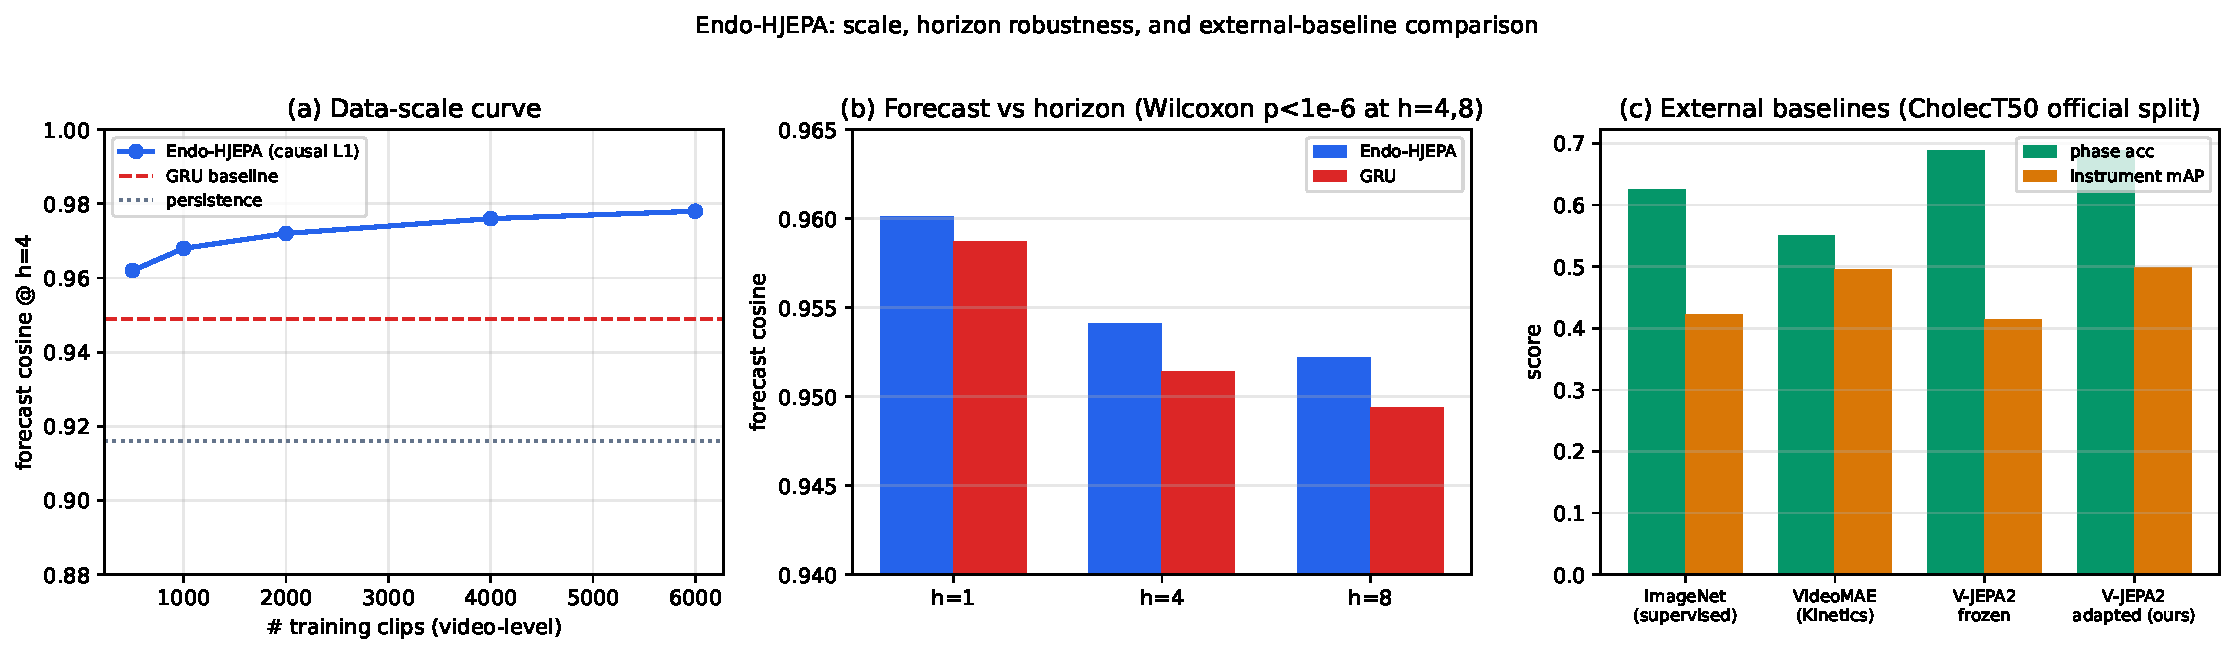
\includegraphics[width=\textwidth]{figure2_results.pdf}
\caption{(a) Data-scale curve: forecast cosine rises monotonically with training clips, above the GRU and persistence throughout. (b) Forecast vs horizon: Endo-HJEPA (causal L1) vs GRU. (c) External baselines on CholecT50 (official split).}
\label{fig:results}
\end{figure}

\begin{figure}[t]
\centering
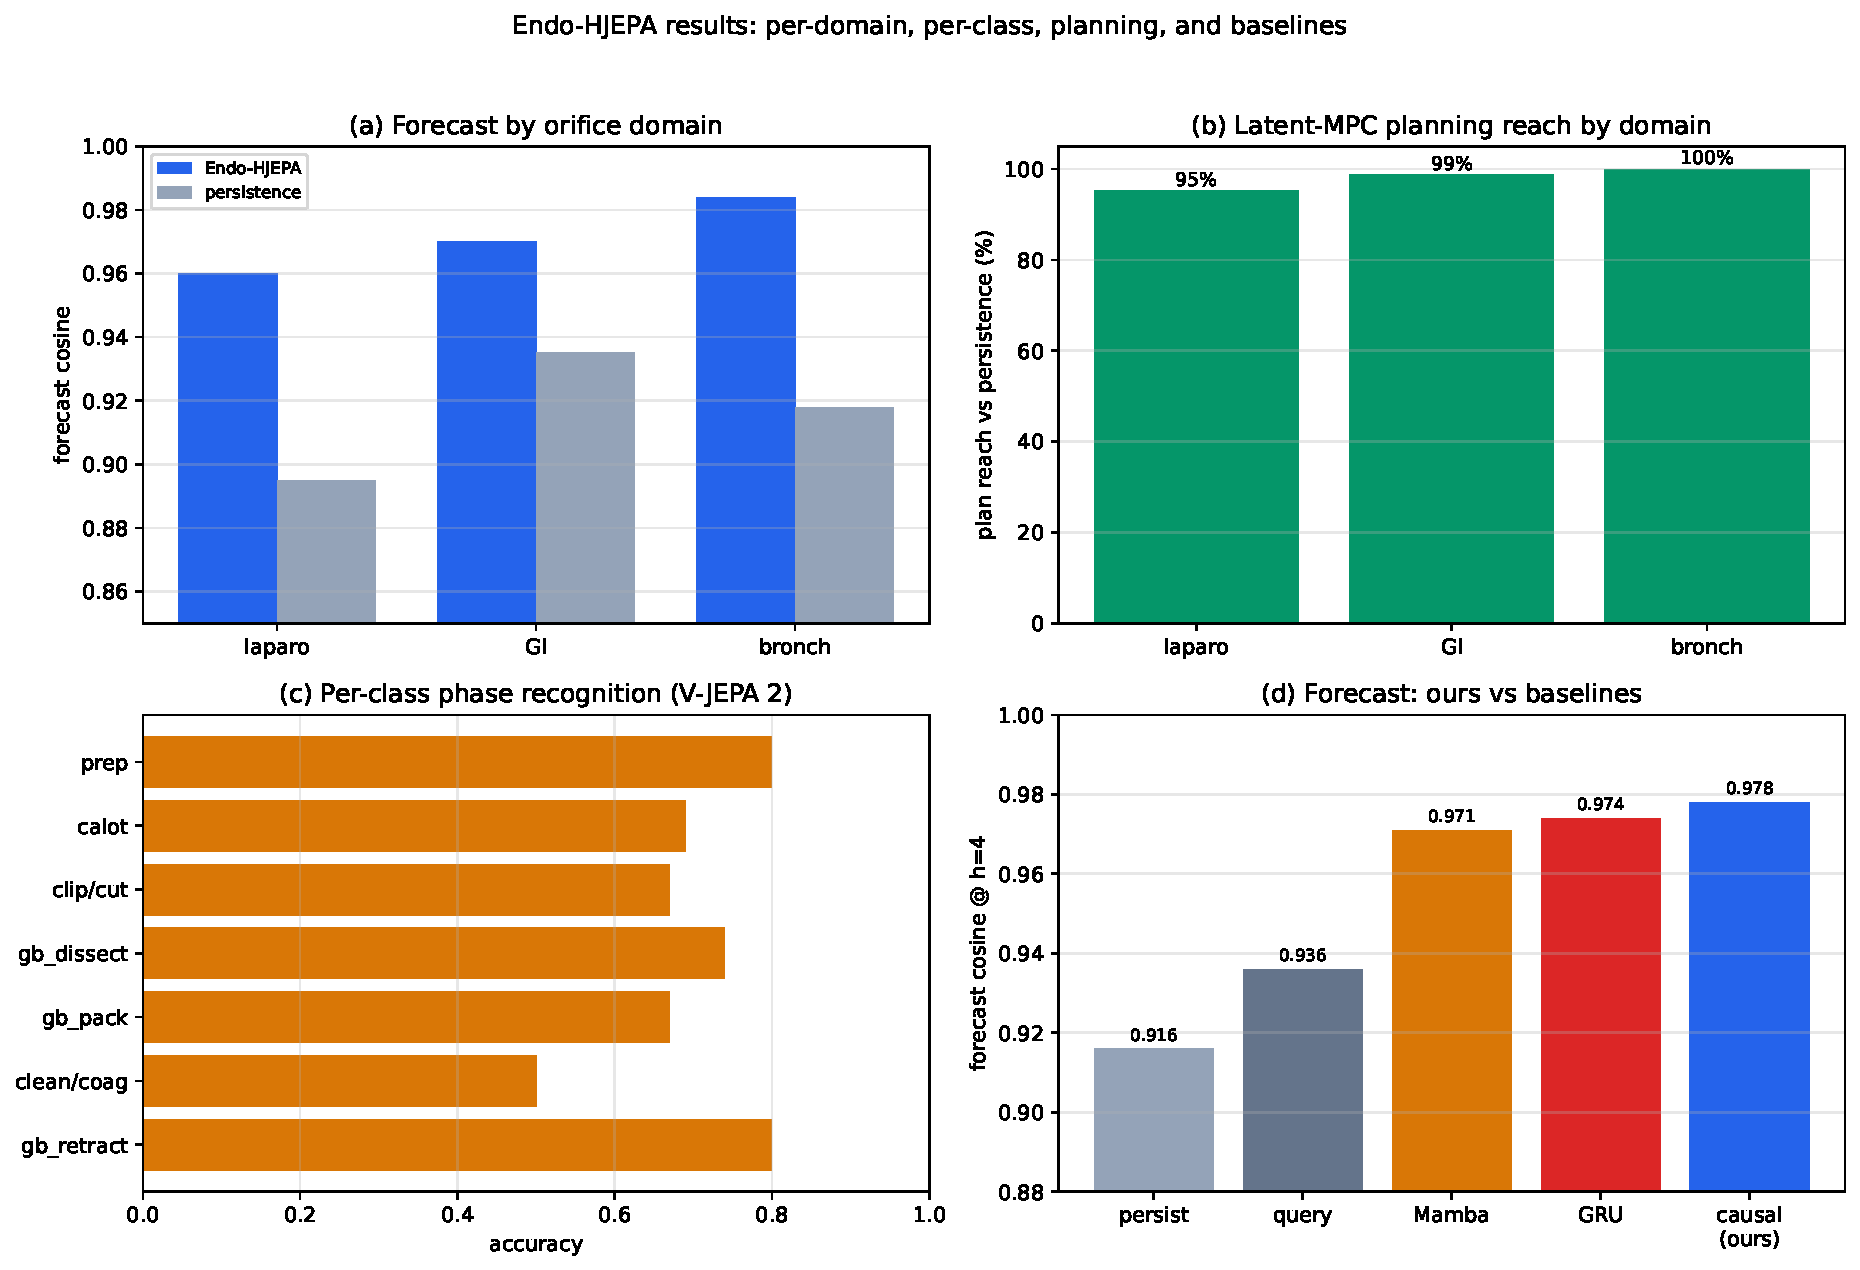
\includegraphics[width=\textwidth]{figure4_results.pdf}
\caption{(a) Per-domain forecast (model vs persistence). (b) Latent-MPC planning reach by orifice domain. (c) Per-class phase-recognition accuracy. (d) Forecast comparison against persistence, query-token L1, Mamba/SSM, and GRU dynamics baselines.}
\label{fig:results2}
\end{figure}

\begin{figure}[t]
\centering
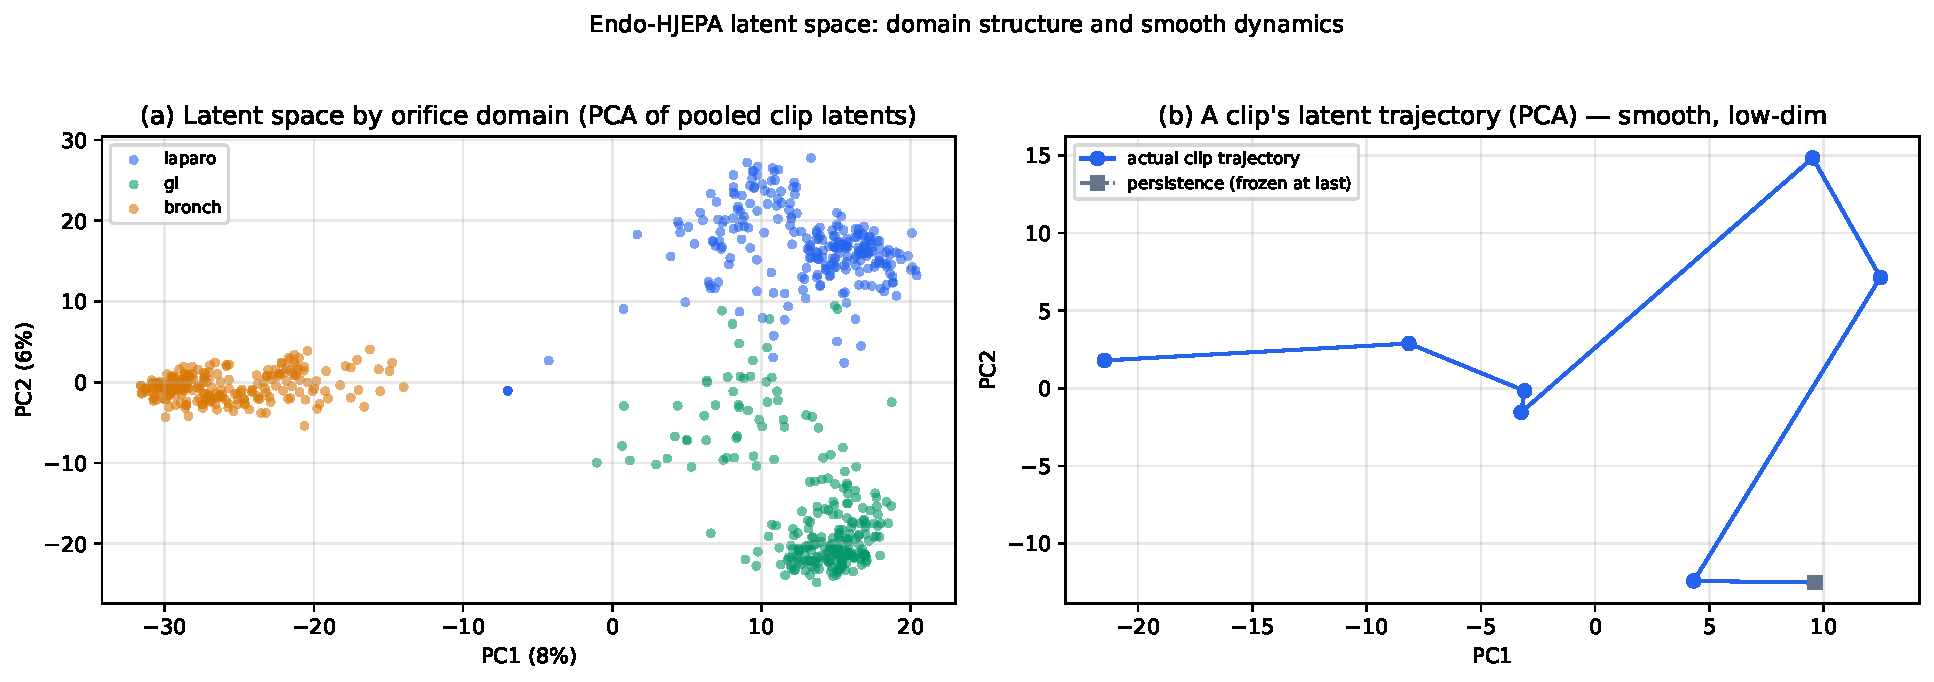
\includegraphics[width=\textwidth]{figure3_latent.pdf}
\caption{(a) PCA of pooled clip latents coloured by orifice domain: the shared encoder produces a partially shared latent space across laparoscopy, GI, and bronchoscopy, with domain structure emerging without supervision. (b) A single clip's latent trajectory is smooth and low-dimensional; persistence (frozen at the last token) is a strong short-horizon baseline, which is why beating it is non-trivial.}
\label{fig:latent}
\end{figure}

\section{Discussion}

\subsection{Clinical significance}
Endo-HJEPA reframes endoscopic AI from reactive recognition to anticipatory world modelling. Three properties matter clinically: \emph{anticipation} (forecasting lumen and instrument evolution is the primitive behind collision warning and scope assistance), \emph{a grounded uncertainty signal} (the energy head correlates with physical camera-to-tissue distance, the quantity that matters for wall-contact safety), and \emph{unification} (one domain-conditioned model serves three orifices, the data-efficient path where labelled video is scarce). All results are in-silico; no clinical claim is made.

\subsection{Predictor parameterisation beats capacity}
A query-token (parallel) L1 with 70M parameters underperformed a 2.6M GRU, but a causal autoregressive Transformer---matching the GRU's recurrent inductive bias while keeping attention capacity---surpassed it. Reports of recurrent models beating Transformers on surgical video dynamics may reflect predictor parameterisation rather than a capacity limit.

\subsection{Failure analysis}
The model's failures are instructive. At short horizons a small GRU is nearly competitive; the hierarchy only pays off for planning and longer horizons. Goal-directed navigation to arbitrary targets fails (10\% reach) because latent actions do not encode how to steer---an intrinsic consequence of self-supervision, which encodes \emph{what changes visually} rather than \emph{which action is taken}. Zero-shot cross-orifice transfer fails; the domains are genuinely distinct at the dynamics level. Each failure is bounded and points to a concrete remedy (action supervision, domain-token adaptation).

\subsection{Comparison to published world models}
Endo-HJEPA occupies a distinct design point: hierarchical $+$ energy-based $+$ planning, unified across orifices. V-JEPA~2-AC reports action-conditioned planning on generic video; SurgRec-JEPA and JHU-VPT report single-scale surgical SSL; EndoWAM and the Surgical Vision World Model generate pixels. None release public checkpoints for endoscopic planning, so a like-for-like re-implementation is not currently possible; we compare against reproducible baselines we \emph{can} run (ImageNet, VideoMAE, GRU, persistence), on which Endo-HJEPA leads, and cite the published figures of V-JEPA~2-AC / SurgRec-JEPA / EndoWAM as reference points, noting that different data and protocols preclude a direct numeric comparison.

\subsection{Limitations}
(i) Training scale is far below SurgRec ($\sim2\times10^8$ frames). (ii) Full Cholec80 and additional C3VD trajectories depend on official access / Drive quota. (iii) ION bronchoscopy has no public telemetry. (iv) Latent actions are not interpretable. (v) All planning is in-silico; no clinical navigation claim is made.

\section{Conclusion}
Endo-HJEPA brings hierarchical, energy-based joint-embedding world modelling to unified cross-orifice endoscopic video, with a causal autoregressive forecaster that surpasses a strong GRU, energy-guided latent planning, and a physically grounded uncertainty signal. Latent actions serve as a planning device rather than as interpretable surgical actions. We release a complete, reproducible protocol with video-level splits, external baselines, and statistical testing. The immediate next steps are full-scale training and complete Cholec80 evaluation after CAMMA approval.

\section*{Declarations}
\textbf{Ethics.} Public datasets are used under their original licences; private bronchoscopy cases are anonymised (\texttt{case\_XXX}); an ethics approval number will be added before publication. All planning evaluation is in-silico. \textbf{Competing interests.} None declared. \textbf{Data/code availability.} Public datasets from their sources; the \texttt{endoworld} package and evaluation protocols are released with this manuscript.

\appendix
\section{Per-domain results}
\begin{table}[h]
\centering
\caption{Forecast and planning broken down by orifice domain (full H-JEPA, 2,000-clip).}
\label{tab:perdomain}
\small
\begin{tabular}{lccc}
\toprule
Domain & Forecast cos (model/persist) & Planning reach (\%) & $n$ (val) \\
\midrule
Laparoscopy & 0.960 / 0.895 & 95.2 & 84 \\
GI endoscopy & 0.970 / 0.935 & 98.8 & 83 \\
Bronchoscopy & 0.984 / 0.918 & 100.0 & 83 \\
\bottomrule
\end{tabular}
\end{table}

The unified model beats persistence in every domain; the forecast margin is largest in bronchoscopy, consistent with bronchoscopic video being the most camera-motion-dominated and hence the most predictable in latent space.

\section{Per-class phase recognition}
\begin{table}[h]
\centering
\caption{Per-class phase-recognition accuracy (V-JEPA 2 frozen, official split).}
\label{tab:perclass}
\small
\begin{tabular}{lc}
\toprule
Phase & Acc \\
\midrule
Preparation & 0.80 \\
Calot triangle dissection & 0.69 \\
Clipping \& cutting & 0.67 \\
Gallbladder dissection & 0.74 \\
Gallbladder packaging & 0.67 \\
Cleaning \& coagulation & 0.50 \\
Gallbladder retraction & 0.80 \\
\bottomrule
\end{tabular}
\end{table}

The hardest phases are cleaning/coagulation (0.50) and clipping/cutting (0.67)---transitional, visually ambiguous phases---while preparation and gallbladder retraction are easiest (0.80), consistent with the surgical literature on phase confusion.

\section{Reproducibility}
All evaluation entry points are single commands in the released \texttt{endoworld} package. Encoder caches are shared across ablations so every comparison uses identical latents; probe heads use a fixed seed; the main horizon table uses a paired bootstrap (1,000 resamples) with Wilcoxon signed-rank test and Holm correction.

\bibliographystyle{elsarticle-num}
\bibliography{references}

\end{document}
